\documentclass[journal, a4paper]{IEEEtran}

%\usepackage{cite}
\usepackage{graphicx}
%\usepackage{psfrag}
%\usepackage{subfigure}
\usepackage{url}
%\usepackage{stfloats}
\usepackage{amsmath}
%\usepackage{array}
\usepackage{gensymb}

% Package Settings
\graphicspath{ {../images/} }

\begin{document}

% Define document title and author
\title{Increased Transcriptional Effects through Polyplex and iCRT in the Presence of Immunological Transcripts}
\author{Austin Mitchell Vecchio
\thanks{Advisor: Dipl.--Ing.~Michelle Ammerman, Lehrstuhl f\"ur Nachrichtentechnik, TUM, WS 2050/2051.}}
\maketitle

% Write abstract here
\begin{abstract}
  To further investigate a larger yield in transfection for non viral gene therapy methods, this experiment
  aims at studying the effects of polyplex treated cells for 6 hours and 24 hours, both with and without iCRT
  against immunological transcripts Interferon-$\alpha$ and Interleukin6. This analysis was conducted through
  reverse transcribing mRNA in human prostate cells and amplifying the resulting complementary DNA through PCR.
  In this experiment, it was seen that polyplex treated cells alone would inhibit the genetic expression of
  the transfected prostate cells as these cells include foreign DNA. However, the addition of iCRT reverses
  the known effect and increases transcription of the prostate cell line above basil levels. Thus, iCRT should
  be investigated as an effective modification to standard non viral gene therapy procedures.

\end{abstract}

% Each section begins with a \section{title} command
\section{Introduction}
  \PARstart{G}{ene} therapy is an experimental method for treating disease by introducing a healthy copy of a
  defective gene into the patient's cells to alter the patients genetic material.
  The alternative is  non viral gene therapy which is a method that can often have simple and large scale production
  with low host immunogenicity. However, non viral gene therapy can often yield low transfection efficiencies.
  This low yield is often due to the inate immune response. The inate immune response is an immune feedback mechanism
  that reacts to foreign DNA (often by viruses or bacteria) through cytokines that rejects the foreign DNA through one of three possibilities.
  These possibilities include: inducing cell death, halting the production of protien or recruiting immune cells to initiate an adaptive immune
  response (e.g. antibody protection). New advances in technologies have improved transfection efficiency by modifying cytokines. Cytokines
  are small protiens that are involved in various types of cell signaling. Classifications of these signalings
  include interferos, chemokines and interleukins. This experiment aims to see if the inate immune response can be inhibited or manipulated
  to improve gene therapy treatments.

  In this experiment, the human prostate cell line will be used for studying the simulated effects of this modified treatment. Prostate cells provide a glandular function
  in the body by generating fluid which serves several functions in reproduction.
  This process will be carried out by nanoparticles that are formed by the self-assembly of DNA/RNA and cationic polymers
  called polyplexes. Polyplexes are specifically designed to deliver foreign genetic material to cells where the cells will incorporate
  the foreign DNA into its own genomic DNA in a process known as transfection.
  The analysis will focus on quantifying the transfection of foreign
  mRNA that will be produced through the prostate cells to determine the effectiveness of this modified treatment.

  Reverse Transcriptase (RT)qPCR is a technique used to describe the level of genetic expression is occuring in vitro
  by measuring the amount of mRNA within a sample. In this technique, mRNA is reverse transcribed in to complementary DNA by
  an enzyme labeled reverse transcriptase.
  For the Real Time PCR experiment, since it is impossible to eliminate all genomic DNA from the cDNA synthesis, two solutions will be prepared.
  The first solution will be a +RT which will include reverse transcriptase and thus, will have cDNA.
  The second solution will be a -RT solution which will lack reverse transcriptase.
  When QtPCR is performed on the -RT solution, genomic DNA will be amplified and will be seen in the resulting data.
  In this experiment, $\beta$-actin and RPL13A will be used for direct controls against the immunological transcripts.
  INF$\beta$ will not be used as it will only appear after cycle 40 in the experiment producing undesirable results.
  The No Template Control will consist of DEPC water.
  The immunological transcripts that will be used in this experiment are Interleukin-6 (IL6) and Inferon-$\alpha$ (INF$\alpha$)
  Beta actin is a type of actin isoform which is highly involved in cell motility, structure and integrity.
  RPL13A is a gene that codes for the 60S ribosomal L13a protein. iCRT will also be present in one polyplex treatment (6hr)
  to test the effects of polyplex when Wnt pathways (cell surface receptors) are inhibited.
  Interleukin-6 (IL-6) is a multifunctional cytokine that defends the host in response to immune and hematopoietic activities.
  Interferon-$\alpha$ is a part of a large subgroup of interferon protiens that help regulate the activity of the immune system.

\section{Methods}
    \subsection{RNA Purification}
      The cells in trizol were thawed before phase separation. During phase separation,
      the poly treated cells in trizol were incubated at 42$^{\circ}$ after which an 0.2mL of chloroform was added per 1mL of Trizol.
      The homoginized sample was incubated at 42$^{\circ}$ for 2-3 minutes following a vigorous shake for 15 seconds.
      The sample was then centrifuged 12,000 g for 15 minutes at 4$^{\circ}$C before transfering the aqueous phase
      to a second tube. (100%) 0.5mL Isopropanol was added to the aqueous phase per 1mL of Trizol used.
      Again, the sample was centrifuged 12,000 g for 15 minutes at 4$^{\circ}$C.
      The pellet was not washed in fear of losing RNA.
      The solution then, underwent a series of centrifuges in between the removal of ethanol to result in an RNA pellet.
      The pellet was then air dried to remove remaining ethanol.
      The pellet was incubated at 42$^{\circ}$ following a resuspension in 20$\mu$L of RNase free water.

    \subsection{cDNA Synthesis}
      For the first step of cDNA Synthesis, two solutions (+RT/-RT) were formed from the following compounds:
      10x dsDNase Buffer, dsDNase, Template RNA, polyplex 24hour RNA and nuclease free water.
      Both solutions were incubated at 42$^{\circ}$ after being centrifuged. The solutions were then chilled on ice, centrifuged and placed back on ice.
      For both solutions, 5X Reaction mix and nuclease free water was added. In the +RT solution, Maxima Enzyme mix (reverse transcriptase) was added to the mixture.
      The -RT solution used DEPC H20 instead of Maxima Enzyme mix so that the -RT solution can simulate the +RT solution without synthesizing RNA into cDNA.
      When the -RT solution undergoes QtPCR, any contaminating genomic DNA will be amplified.
      The two solutions will be then mixed gently and centrifuged. An incubation period will take place at 25$^{\circ}$C for 10 min
      followed by a second incubation session at 50$^{\circ}$C for 15 min.
      The reaction will be terminated by heating the solutions at 85$^{\circ}$C for 5 min.
      This process was conducted using Maxima First Strand cDNA Synthesis Kit with dsDNase (Thermo Scientific, Cat#: K1671)

    \subsection{Qt PCR}
      Each well will contain 10$mu$L of 2X iTaq universal SYBR Green Supermix,
      5$\mu$L of a primer (IL6, INF$\alpha$, $\beta$-actin or RPL13A),
      and 5$\mu$L of the respective diluted cDNA.
      The cDNA needs to be diluted to 4ng/$\mu$L from their respective concentrations before it is added to the wells.
      The concentrations of cDNA for both sets of Poly24 and no washed cells were all around 100ng/ $\mu$ L.
      Therefore only one set of calculations were needed for determining the proper dilution of cDNA into water
      for either INF$\alpha$ and IL6 or $\beta$-actin andRPL13A and the respective -RT wells. For just cells,
      a different set of calculations were needed since the original cDNA concentrations were around 11 ng/ $\mu$ L.
      All wells contained the Green Supermix. The columns were sorted in the following manner:
      1-3 contained IL6, 4-6 contained INF$\alpha$, 7-9 contained $\beta$-acting and 10-12 contained RPL13A.
      Refer to Table II for a compressed map of the PCR wells. The QtPCR was ran for 40 cycles.

    \subsection{Gel Electrophoresis}
      In order to further understand the results gained from the QtPCR, an 1.2% agarose gel was poured
      and gel electrophoresis was ran on the PCR product.

    \subsection{Analysis}
      The results from the QtPCR produced Ct values from each well.
      A Ct value is a numeric inverse correlation to the quantity of nucleic acid detected by the aparatus.
      Comparisons are made between Polyplex treated cells for 24 hours version [AV], Polyplex treated cells for 24 hours version [Ts],
      Polyplex treated cells for 6 hours with iCRT, Cells that were not washed after 6 hours, cells that were not washed and just cells.
      Each comparison was conducted by taking the difference between the Ct values of the two primers (immunological transcript minus control)
      on two different treatments. A second difference was taken between these two treatments (i.e. Poly24-NoWash) and then applied to the $\Delta$\Delta$ct method
      to determine the fold induction. This was repeated three times, and thus an average was determined.

\section{Results}

  \subsection{QtPCR}

  It can be seen in Table I that both the Poly24[AV] and Poly24[Tk] variants compared to unwashed cells
  exhibits fold induction values in the range of $10^{-5}$. This can also be seen in Figures 2,3,4 and 5.
  Processing this value by using a $log_2$ scale will explain that the polyplex treatment at 24 hours
  against unwashed cells inhibits genetic transcription levels at a factor of 16.

  When comparing Poly24[AV] and Poly24[Tk] variants against washed cells,
  the resulting fold induction values were at a rate of $10^{-2}$. Processing this value
  by using a $log_2$ scale will explain that the polyplex treatment
  in this case against washed cells inhibits transcription levels at a factor of 6.6

  The addition of iCRT to Polyplex at a treatment of only 6 hours against unwashed
  cells at six hours exhibits a fold induction values at a rate of $10^2$. Processing
  this value using a $log_2$ scale will explain that the polyplex treatment under these
  conditions increased transcription levels at a factor of 6.6

  As previously explained, when viewing the transcription levels of just cells
  against unwashed cells, a large difference in transcription levels can be seen.

    \begin{table}[!hbt]
      % Center the table
      \begin{center}
      % Fold Inductions
      \caption{QtPCR Fold Inductions}
      \label{tab:simParameters}
      % Table itself: here we have two columns which are centered and have lines to the left, right and in the middle: |c|c|
      \begin{tabular}{|c|c|c|c|c|}
        \hline
        & IL6-$\beta$-act. & IL6-RPL. & INF$\alpha$-$\beta$-act. & INF$\alpha$-RPL. \\
        \hline
        Poly24[AV]-NoWash & 3.85E-05 & 7.58E-03 & 5.09E-05 & 1.05E-02 \\
        \hline
        Poly24[AV]-Cells & 3.10E-02 & 3.54E-02 & 3.94E-02 & 4.27E-02 \\
        \hline
        NoWash-Cells & 8.01E+02 & 4.65E+00 & 7.01E+02 & 4.08E+00 \\
        \hline
        Poly24[Ts]-NoWash & 8.20E-05 & 4.64E-03 & 3.77E-05 & 6.04E-03\\
        \hline
        Poly24[Ts]-Cells & 6.54E-02 & 5.90E-02 & 2.57E-02 & 2.55E-02\\
        \hline
        Poly6+iCRT-NoWash6 & 5.00E+2 & 4.21E+2 & 2.58E+1 & 2.23E+1 \\
        \hline
      \end{tabular}
      \end{center}
    \end{table}

  \subsection{Gel Electrophoresis}

    Refering to Figure 1, it can be seen that the selections of PCR products was based off of melt curves that were inconsistent with
    surrounding wells of similar product (i.e. $\beta$-actin for just cells).
    Lanes 2-4 (Wells: E1,E2,E3,G1) consists of -RT solutions. These lanes are empty displaying
    genomic DNA that is almost undetectable. Lane 8 (Well A5) displays a lack of cDNA
    for Interferon-$\alpha$ where there should exist amplified cDNA. Lanes  7,9,11 and 14
    (Wells: C1,C4,D10,A8) are displaying bands at a greater illumination compared to other lanes.
    Lanes 7 and 9 consist of Just Cells in Interleukin-6 and Interferon-$\alpha$ respectively.
    Lanes 11 and 14 are polyplex cells treated for a 24 hour duration in both the [AV] and [Ts] variants
    for RPL13A and $\beta$-actin respectively.
    Lanes 6,12, and 13 contain smaller amounts of cDNA compared to Lanes 7,9,11 and 14 as they do not contain
    as great illumination.
    Lane 6 (Well B1) is cells that were not washed for Interleukin 6.
    Lanes 12 and 13 (Wells: E11,E12) consist of -RT solutions for RPL13A displaying amplified genomic DNA.

  \section{Discussion}

    As seen in Table 1, both the Poly24[AV] and Poly24[Tk] variants express lower transcription rates
    than either just cells or unwashed cells in the presence of an immunological response.
    A similar result was explained by the research conducted at University of Michigan (Matz, R. L. 2013).
    The resulting value does depend upon if the control cells were washed or unwashed, which control
    protien was compared against and which immunological response was used. In all cases the
    polyplex treatment at 24 hours alone inhibits genetic transcription.
    This relationship can be seen in Figures 2,3,4 and 5. However,
    the addition of iCRT in the treatment compared against the nowash at both six hour long treatments
    displays a positive growth in transcription levels. This can also be seen in figures 2-5 as the
    only rate comparsion (that is not a control) shows a positive correlation. This would suggest that polyplex alone
    would only inhibit transcription rates, but paired with iCRT or something of a similar nature
    increases transcription from a basil level. This would need to be further investigated.
    As seen in the figures (2-5), the comparsion between washed and uwashed cells also shows a postive correlation
    explaining increased transcription levels. It is possible that the washed cells
    clears out the chemical treatment that would inhibit transcription rates. If so, a secondary
    control may need to be used when running this experiment again.
    This can also be verified through the agarose gel of Figure 1. Lanes 7 and 9
    that consist of just cells with an immunological transcript should yield normal
    transcription rates as the plain cell line should not be effected by an immunological response.
    However, lanes 11 and 14 are polyplex treated cells for 24 hours tested against the control protiens.
    Since the polyplex treated cells are not combined with an immunological indicator, transcription
    rates would not be inhibited and thus, normal transcription rates are seen.
    Lane 8 displays a lack of cDNA as it is a polyplex treated cell for 24 hours in the presence
    of Interferon-$\alpha$. This further verifies the statement that polyplex alone will inhibit genetic transcription.

  \section{Conclusion}

    Polyplex treatment by itself will only further inhibit transcription rates in the presence of an immunological response.
    However, the addition of iCRT to the treatement created a scenario where polyplex increased the
    transcription rates. The usage of iCRT in the treatment provides insight that may yield promising results towards
    a more stable version of non viral gene therapy. No conclusion was able to be derived from the timeframes of 6 hour
    and 24 hour treated polyplex. Thus, to futher understand the nature polyplex and iCRT treated cells in response to a specific duration,
    it would be suggested that the polyplex cells are treated in 3 hour increments from 3 hours to 24 hours both with and without iCRT.

  \begin{table}[!hbt]
    % Center the table
    \begin{center}
    % Fold Inductions
    \caption{PCR Wells for Controls}
    \label{tab:simParameters}
    % Table itself: here we have two columns which are centered and have lines to the left, right and in the middle: |c|c|
    \begin{tabular}{|c|c|c|c|c|c|c|c|c|c|c|c|c|c|}
      \hline
      & Primer & 1/4/7/10 & 2/5/8/11 & 3/6/9/12 \\
      \hline
      A & Poly24[Tk] & 4ng/$\mu$L & 4ng/$\mu$L & 4ng/$\mu$L\\
      \hline
      B & Just Cells & 4ng/$\mu$L & 4ng/$\mu$L & 4ng/$\mu$L\\
      \hline
      C & No Wash & 4ng/$\mu$L & 4ng/$\mu$L & 4ng/$\mu$L\\
      \hline
      D & Poly24[AV] & 4ng/$\mu$L & 4ng/$\mu$L & 4ng/$\mu$L\\
      \hline
      E & -RT & Poly24[Tk] & Cells & Poly24[AV] \\
      \hline
      E & NTC & Poly24[Tk] & Cells & Poly24[AV] \\
      \hline
      G & & NoWash(-RT) & NoWash(NTC) &\\
      \hline
      H & & & &\\
      \hline
    \end{tabular}
    \end{center}
  \end{table}

  \begin{table}[!hbt]
    % Center the table
    \begin{center}
    % Fold Inductions
    \caption{List of Primers}
    \label{tab:simParameters}
    % Table itself: here we have two columns which are centered and have lines to the left, right and in the middle: |c|c|
    \begin{tabular}{|c|c|c|}
      \hline
      Primer Name & Tm & Sequence \\
      RTPCR-IL6-FOR & 60 & CCTTCCAAAGATGGCTGAAA \\
      \hline
      RTPCR-IL6-REV & 60 & CACAGCTCTGGCTTGTTCCT \\
      \hline
      RTPCR-IFNAall-FOR & 61 & GCACCGAACTCTACCAGCAG \\
      \hline
      RTPCR-IFNAall-REV & 60 & ACAACCTCCCAGGCACAA \\
      \hline
      RTPCR-B-Actin-FOR & & TTGCCGACAGGATGCAGAA \\
      \hline
      RTPCR-B-Actin-REV & & GCCGATCCACACGGAGTACTT \\
      \hline
      RTPCR RPL13A –FWD & & CCTGGAGGAGAAGAGGAAAGAGA \\
      \hline
      RTPCR RPL13A REV & & TTGAGGACCTCTGTGTATTTGTCAA \\
      \hline
    \end{tabular}
    \end{center}
  \end{table}

% Now we need a bibliography:
\begin{thebibliography}{5}
  \bibitem{Handout}
  Unknown. Elucidating the Innate Immune Response(s) to Non-Viral Gene Therapy. Mol Bio Lab Week 6.

  \bibitem{Article}
  Matz, R. L., Erickson, B., Vaidyanathan, S., Kukowska-Latallo, J. F., Baker, J. R., Orr, B. G., & Holl, M. M. (2013).
  Polyplex Exposure Inhibits Cell Cycle, Increases Inflammatory Response, and Can Cause Protein Expression without Cell Division.
  Mol. Pharmaceutics Molecular Pharmaceutics, 10(4), 1306-1317. doi:10.1021/mp300470d

  \bibitem{Instruction}
  Maxima First Strand cDNA Synthesis Kit for RT-qPCR, with dsDNase. (n.d.). Retrieved from
  https://www.lifetechnologies.com/order/catalog/product/K1671

  \bibitem{Instruction}
  Real-Time PCR Technology Basics. (n.d.). Retrieved from http://biosistemika.com/workshops/qpcr-basics/

\end{thebibliography}

    \begin{figure}[t]
      \centering
      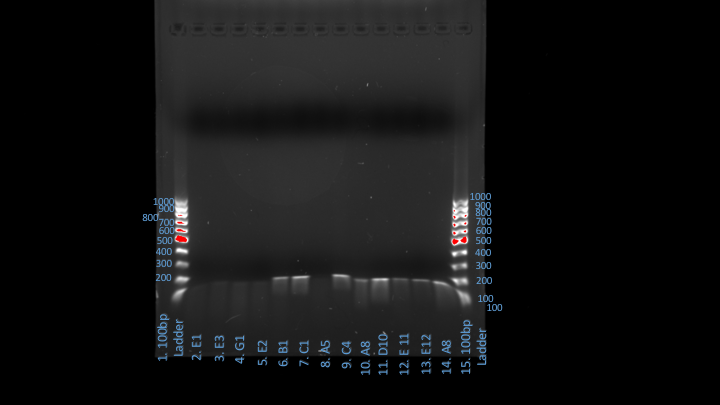
\includegraphics[width=8cm]{supergel}
      \caption{A 1.2\% agarose gel used to further analyze discrepencies seen in the melt curves of the PCR product.}
      \label{fig:mesh1}
    \end{figure}

    \begin{figure}[t]
      \centering
      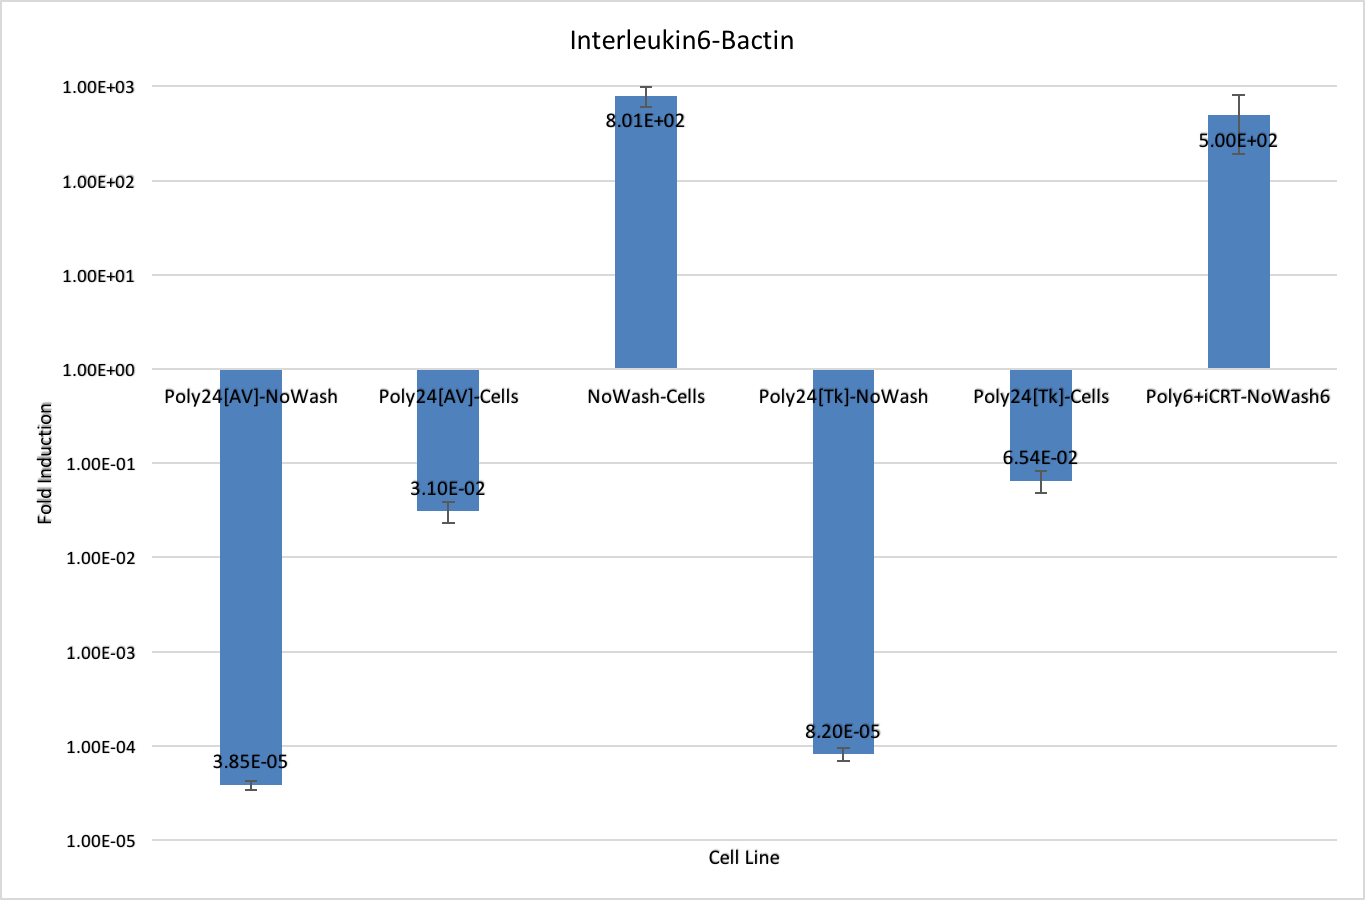
\includegraphics[width=8cm]{il6-bactin}
      \caption{Logarithmic fold Inductions for Interleukin-6 vs $\beta$-actin.
      Refer to the analysis subsection of the methods section for insight on how this graph was constructed.
      }
      \label{fig:mesh1}
    \end{figure}

    \begin{figure}[t]
      \centering
      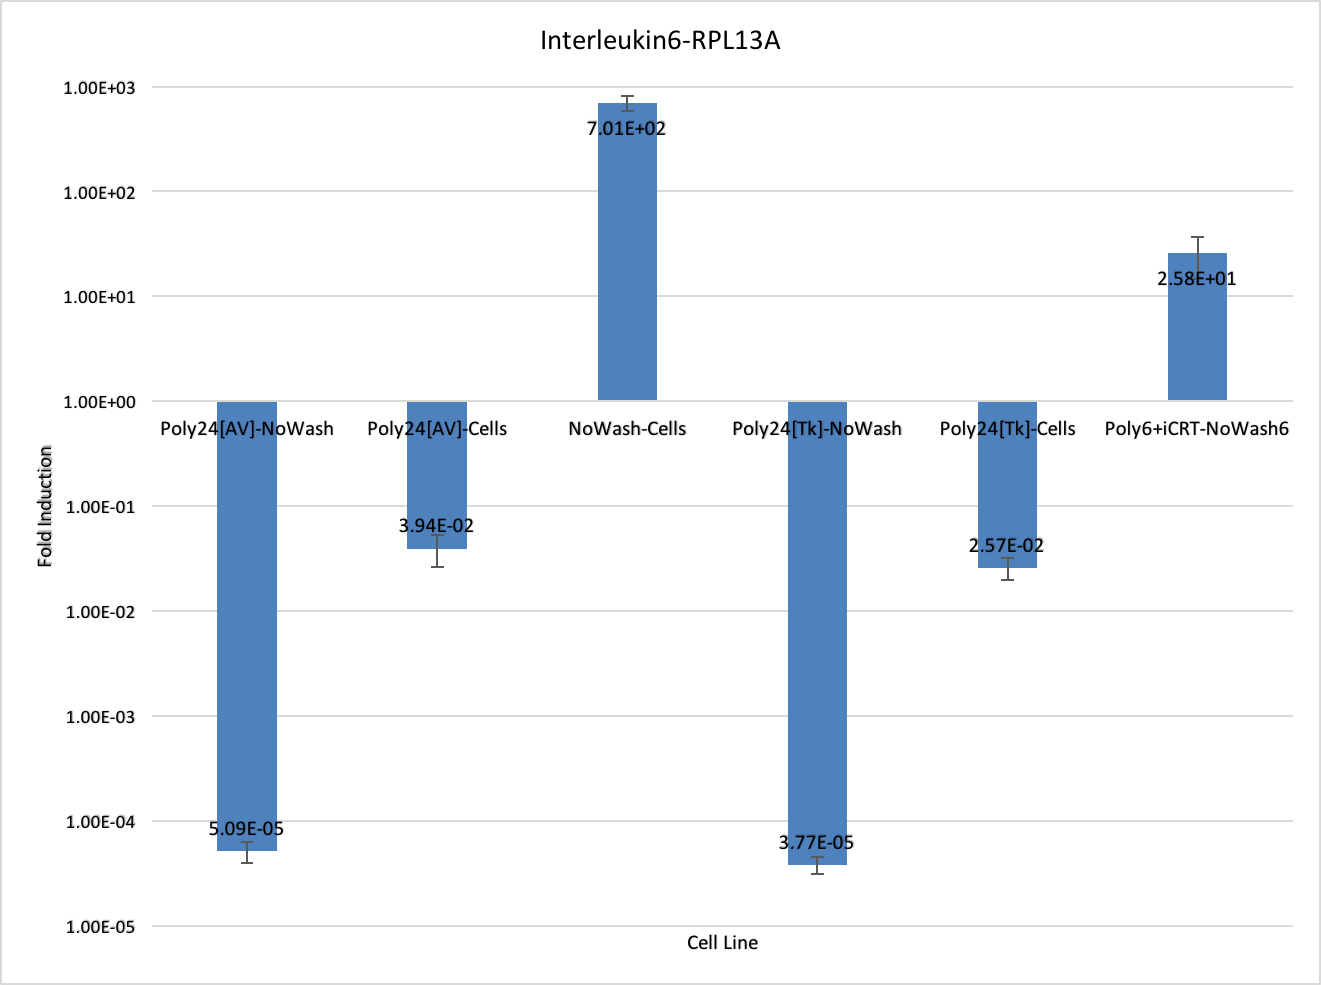
\includegraphics[width=8cm]{il6-rpl13a}
      \caption{Logarithmic fold Inductions for Interleukin-6 vs RPL13A.
      Refer to the analysis subsection of the methods section for insight on how this graph was constructed.
      }
      \label{fig:mesh1}
    \end{figure}

    \begin{figure}[t]
      \centering
      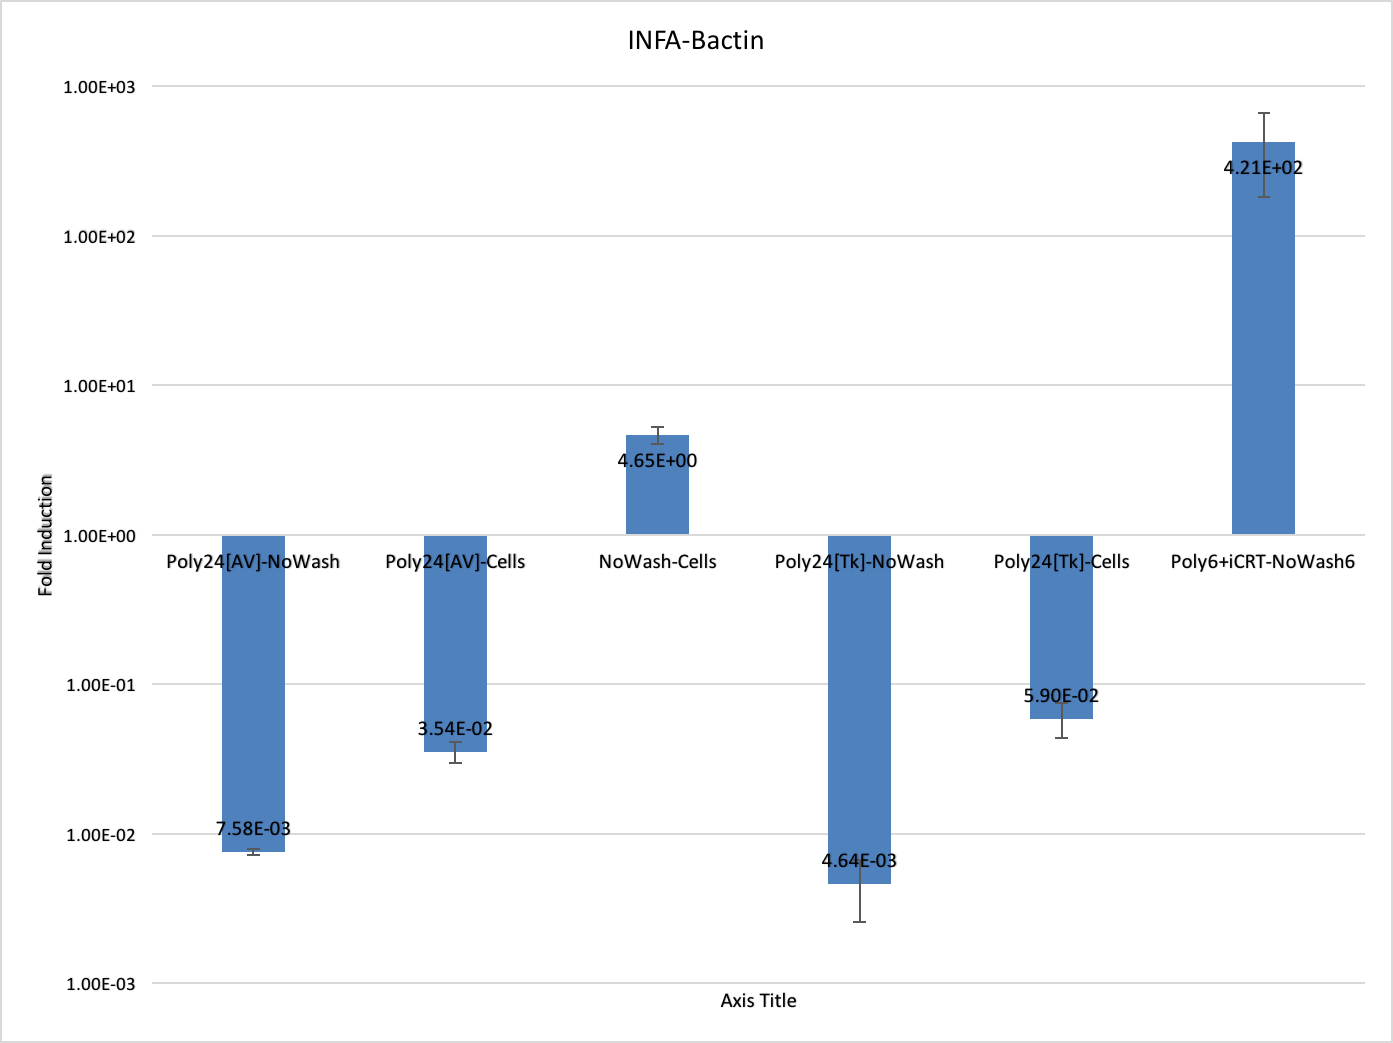
\includegraphics[width=8cm]{infa-bactin}
      \caption{Logarithmic fold Inductions for Interferon-$\alpha$ vs $\beta$-actin.
      Refer to the analysis subsection of the methods section for insight on how this graph was constructed.
      }
      \label{fig:mesh1}
    \end{figure}

    \begin{figure}[t]
      \centering
      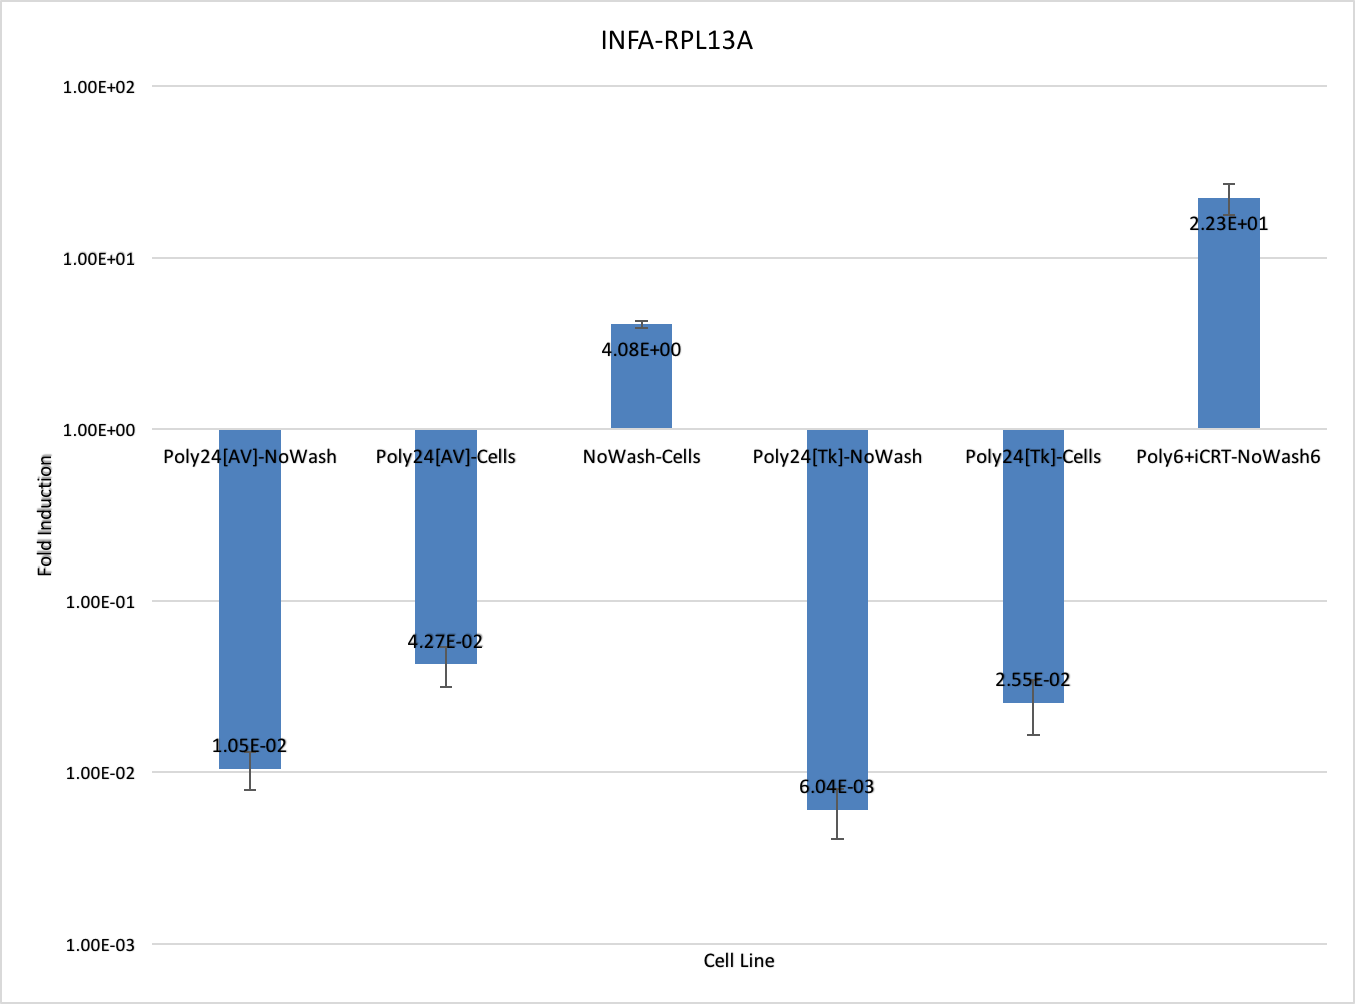
\includegraphics[width=8cm]{infa-rpl13a}
      \caption{
      Logarithmic fold Inductions for Interferon-$\alpha$ an immune cytokine vs RPL13A a standard protien.
      Refer to the analysis subsection of the methods section for insight on how this graph was constructed.
      }
      \label{fig:mesh1}
    \end{figure}
% Your document ends here!
\end{document}
